\documentclass[11pt]{article}
\usepackage[margin=1in]{geometry}
\usepackage{graphicx,booktabs,amsmath,hyperref}
\title{GLAM on the offline $\beta(\rho)$ curve:\\ r24, r24m, r24m2 and r24m3}
\author{Aidan Gettemy}
\date{November 9, 2026}
\begin{document}
\maketitle

\section{Summary}
All four runs use 24 chains, 40\,000 iterations, $\sigma_{\rm conc}=0.002$, $\sigma_{\rm dp}=0.004$ and target acceptance 0.25; statistics are over the tail after iteration 14\,000. r24 restarts every chain near one anchor; r24m, r24m2 and r24m3 keep an open archive of anchors. r24m3 changes the archive and the schedule at once: stages of 1000 (global) and 500 (local) iterations instead of 200, $\varepsilon=0.01$, $\alpha=0.7$, gain scale 8, minimum score 0.5, minimum anchor distance 12, cap 300, quality tolerance 400, exploit/frontier/explore fractions 0.10/0.35/0.55, a frontier target $\Phi=800$ and a restart $\Phi$-tolerance of 50 with 10 attempts.
\begin{itemize}
\item \textbf{Archive selection now works.} The 0.5 cut-off bound at most exchanges after iteration 5\,500 (10--30 admissible candidates rejected, lowest selected score 0.50--0.51). The log-det novelty of the selected anchors fell from 0.76 to 0.49 instead of sitting at 1. The archive reached 231 anchors (265 eligible) and never hit the cap of 300. Its effective rank rose to 13.7 (4.6 in r24m2).
\item \textbf{Descent is slower.} The best anchor ended at $\Phi=957$ (r24 738, r24m2 839, r24m 890) and was still falling; all 24 chains slide down together to the end of the run (Figure~\ref{fig:phi}). The concentration misfit is the largest of the four runs.
\item \textbf{Uncertainty is better calibrated, but the tail is not stationary.} Coverage rose from about 0.28/0.52 (1$\sigma$/2$\sigma$) to 0.43/0.73 and the rms $z$-score fell from about 3.3 to 2.0. Part of that spread is the downward drift inside the window, not posterior width: MPSRF is the worst of the four runs (block 0 never reaches 1.2).
\item \textbf{The frontier never found a region.} Frontier tracking was active at every exchange, but \texttt{successful\_region\_count} stayed 0, because the target $\Phi=800$ was never reached.
\end{itemize}

\section{Fit and field comparison}
\begin{table}[h]\centering
\begin{tabular}{lrrrr}\toprule
 & r24 & r24m & r24m2 & r24m3 \\ \midrule
Best anchor $\Phi$ at the end & 738 & 890 & 839 & 957 \\
Median anchor $\Phi$ at the end & 738 & 924 & 907 & 1156 \\
RE$_{\rm conc}$, mean & 0.0841 & 0.0916 & 0.0900 & 0.0995 \\
RE$_{\rm conc}$, 5--95\% & 0.077--0.094 & 0.086--0.099 & 0.084--0.100 & 0.090--0.113 \\
RE$_{\rm dp}$, median & 0.00235 & 0.00228 & 0.00218 & 0.00307 \\
Tail acceptance, global / local & 0.219/0.219 & 0.218/0.223 & 0.220/0.233 & 0.221/0.229 \\
\midrule
Field corr., best sample & 0.650 & 0.589 & 0.580 & 0.570 \\
Field corr., posterior mean & 0.648 & 0.609 & 0.591 & 0.623 \\
RMSE ($\ln K$), best sample & 0.779 & 0.837 & 0.849 & 0.851 \\
RMSE ($\ln K$), posterior mean & 0.765 & 0.794 & 0.816 & 0.766 \\
Coverage 1$\sigma$ / 2$\sigma$ & 0.277/0.516 & 0.303/0.544 & 0.261/0.491 & 0.433/0.725 \\
rms $z$-score & 3.37 & 3.29 & 3.41 & 2.01 \\
Mean posterior sd of $\ln K$ & 0.274 & 0.305 & 0.278 & 0.438 \\ \bottomrule
\end{tabular}
\caption{Fit and field statistics (\texttt{diagnostics.json}, \texttt{field\_comparison.json}; tail after iteration 14\,000). The reference field has sd$(\ln K)=0.966$. One run per configuration, so small differences could come from the seed.}
\end{table}
The posterior mean of r24m3 is as accurate as that of r24 (RMSE 0.766 versus 0.765) and better than r24m and r24m2; its best single state is the least accurate. The data fit is the worst of the four runs, as expected from the higher $\Phi$.

\begin{figure}[h]\centering
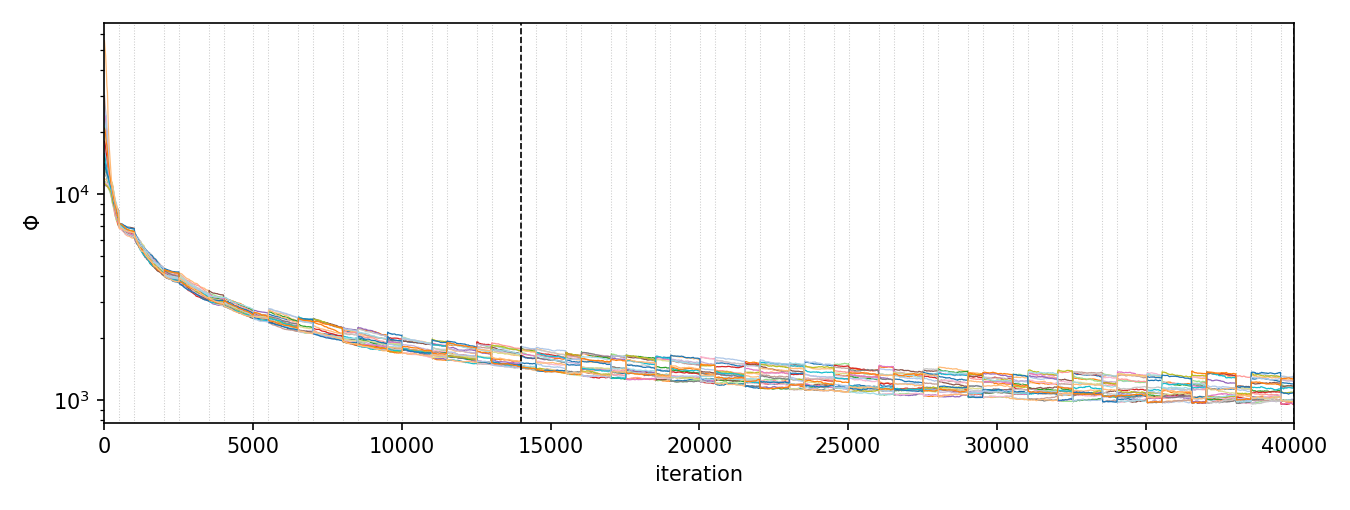
\includegraphics[width=0.95\textwidth]{fig_traces_phi_r24m3.png}
\caption{r24m3: $\Phi$ of all 24 chains versus iteration (log axis). The dashed line is the end of adaptation (iteration 14\,000), where the post-processing window starts. The chains are still descending at iteration 40\,000.}\label{fig:phi}
\end{figure}

\section{Archive}
\begin{figure}[h]\centering
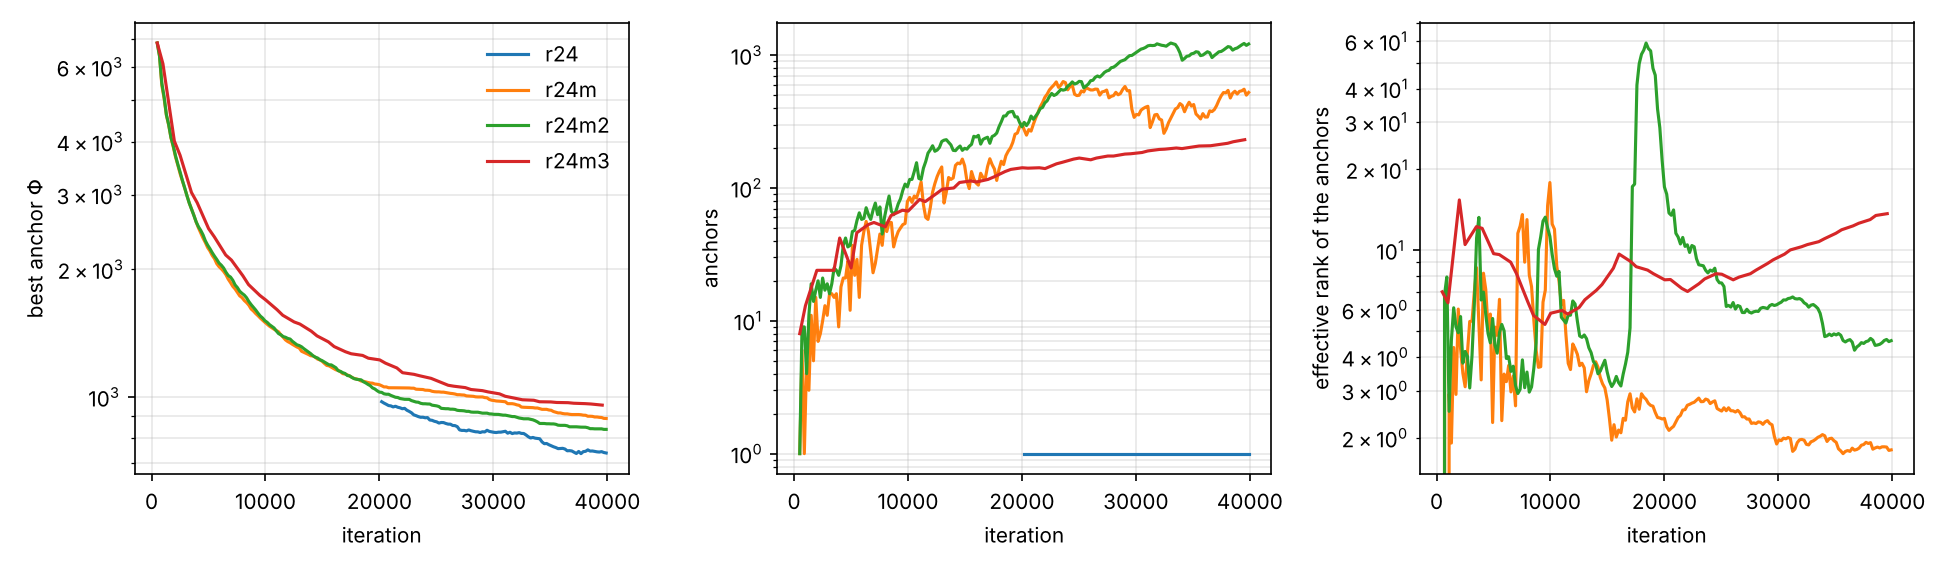
\includegraphics[width=\textwidth]{fig_archive.png}
\caption{Best anchor $\Phi$, archive size and effective rank of the anchor covariance at every exchange. r24 has one anchor (no effective rank), and its exchange history starts at iteration 20\,000 because it ran in two pieces.}
\end{figure}
\begin{table}[h]\centering
\begin{tabular}{lrrrr}\toprule
 & r24 & r24m & r24m2 & r24m3 \\ \midrule
Exchanges & 99 & 197 & 197 & 53 \\
Anchors at the end & 1 & 524 & 1214 & 231 \\
Largest archive & 1 & 633 & 1234 & 231 \\
Effective rank at the end & --- & 1.8 & 4.6 & 13.7 \\ \bottomrule
\end{tabular}
\caption{Archive size and effective rank (\texttt{exchanges.csv}).}
\end{table}
In r24m3 the selection settings do what they were set to do: the score cut-off bounds the archive, log-det novelty is no longer saturated, and the effective rank is the highest of the three multi-anchor runs. The archive size is still set mostly by candidate supply (231 selected of 265 eligible). With only 53 exchanges the archive had few chances to grow.

\section{Convergence diagnostics}
\begin{table}[h]\centering
\begin{tabular}{lrrrr}\toprule
 & \multicolumn{4}{c}{final MPSRF} \\
 & r24 & r24m & r24m2 & r24m3 \\ \midrule
$\rho$ (whitened) & 1.000 & 1.003 & 1.004 & 1.014 \\
first 100 coordinates & 1.015 & 1.030 & 1.029 & 1.132 \\
block 0 (500 dims) & 1.069 & 1.107 & 1.101 & 1.474 \\
max per-coordinate PSRF & 1.001 & 1.007 & 1.008 & 1.036 \\ \midrule
 & \multicolumn{4}{c}{iteration at level 1.2} \\
$\rho$ & 15\,200 & 15\,200 & 15\,200 & 15\,885 \\
first 100 coordinates & 16\,392 & 17\,824 & 18\,143 & 31\,262 \\
block 0 & 24\,163 & 27\,890 & 28\,045 & never \\ \bottomrule
\end{tabular}
\caption{MPSRF from iteration 14\,000 (2600 thinned samples per chain). The MPSRF step first failed for r24m3 on an exactly singular within-chain covariance of $\rho$ (frozen during a local stage); \texttt{mpsrf\_curve} now returns NaN for such points.}
\end{table}
\begin{figure}[h]\centering
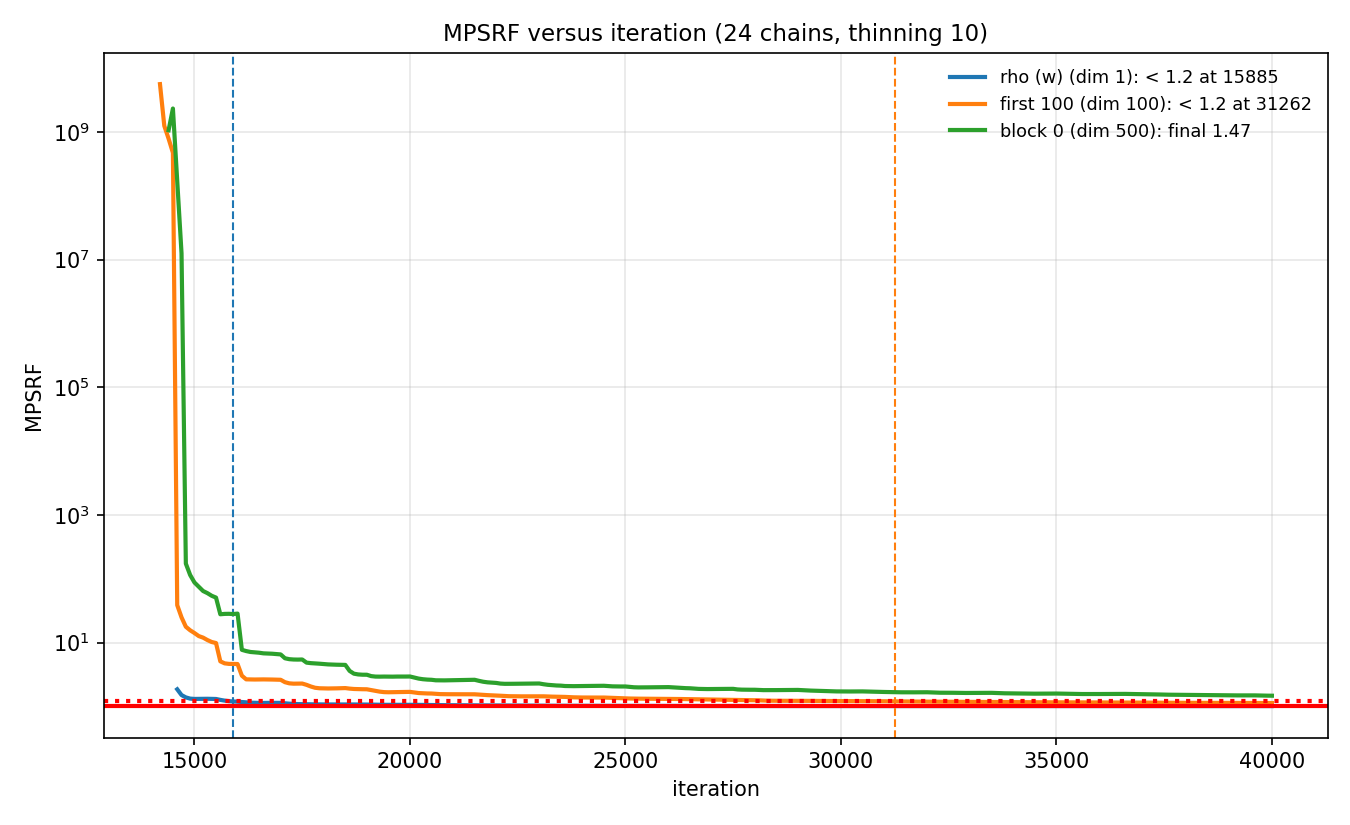
\includegraphics[width=0.8\textwidth]{fig_mpsrf_r24m3.png}
\caption{r24m3: MPSRF versus iteration.}
\end{figure}
Chains agree less in r24m3 than in the earlier runs, for the two reasons above: the restarts spread the chains over more distinct anchors, and all chains are drifting down through the window. This run cannot separate the two.

\section{What follows}
\begin{enumerate}
\item Continue r24m3 beyond 40\,000 iterations (the descent is still going) and recompute calibration on a later window; if the coverage stays above about 0.4 as $\Phi$ levels off, the spread is real.
\item Raise the exploit share (for example 0.25) and shorten the stages (about 500) to recover descent speed.
\item Set the frontier target where it can be reached (for example 1100--1200 early, lowered later) so the successful-region machinery can act.
\item Use a window start closer to where $\Phi$ plateaus when judging calibration and MPSRF.
\end{enumerate}
\end{document}
